\documentclass[main]{subfiles}
\begin{document}
%@@@@@@@@@@@@@@@@@@@@@@@@@@@@@@
% summarizes lecture 8
% author: 

\section{Photodiodes, photoreceptor}

\subsection{How does the I-V curve of a diode change in the presence of light?}

The current-voltage characteristic of a photodiode has the same
shape as that of a normal diode, but the curve is displaced along the current
axis by the value of the photocurrent (see fig. \ref{fig:photodiode_charac}).

\begin{figure}[htbp]
  \centering
  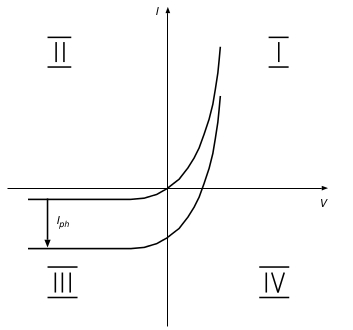
\includegraphics[scale=0.8]{pics/photodiode_charac.jpg}
  \caption{Steady-state current-voltage characteristics of a photodiode. The upper curve is the normal diode characteristic (dark characteristic). The lower curve shows the characteristic under illumination \cite{book:VLSI}.}
  \label{fig:photodiode_charac}
\end{figure} 

In the presence of an applied external bias the (negative) photocurrent  is superimposed onto the diode current.

\subsection{How does phototransduction occur in silicon?}

Transduction means transformation of the energy from one form to another. Phototransduction means transforming from photon to electronic signals \cite{lab8}.

In a semiconductor, an incident photon and therefore its energy can be absorbed by an electron. A
photon with an energy larger than or approximately equal to the bandgap energy can excite an electron from the valence band into the conduction band
(corresponds to the generation of an electron-hole pair). Illumination of a semiconductor therefore increases the concentration of mobile charge carriers (electrons). 

If the motion of the carriers is driven by diffusion, then the
generation is balanced by recombination(creation of pairs).

However, if electron-hole pairs are generated in depletion region and subjected to its built-in electric field, pairs are likely to be separated.  
Some of the separated carriers contribute to an electrical output signal (reverse photo current). The separated mobile charges are "swept home" as the minority charges dominate in depletion region. 

\begin{figure}[htbp]
  \centering
  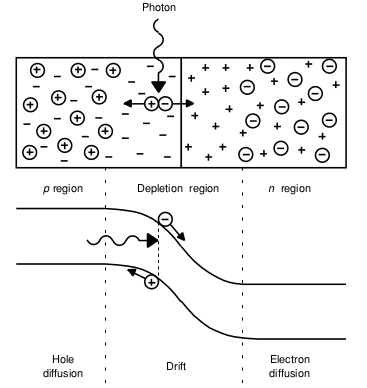
\includegraphics[scale=0.8]{pics/photodiode_principle.jpg}
  \caption{Principle of operation of a photodiode. Electron-hole pairs generated by incident photons in or
within a diffusion length outside the depletion region become separated and contribute to a reverse
generation current \cite{book:VLSI}.}
  \label{fig:photodiode_principle}
\end{figure} 

If the photodiode is open-circuited, that is, no external current is allowed
to flow, then generated charge accumulates at the boundaries of the depletion
region until a steady state is attained. In steady state, a forward diffusion current in
the junction compensates for the photo-
current \cite{paper:photo}.

If the photodiode terminals are short-circuited the photocurrent
can be measured as a reverse diode current. In the presence of an applied ex-
ternal bias the photocurrent is superimposed onto the diode current \cite{book:VLSI}.



\subsection{How you can use adaptation in a feedback loop to cancel out circuit mismatch?}

In the simple source-follower logarithmic photoreceptor circuit (see fig. \ref{fig:photoreceptor_log}) in real world application there are two important problems: mismatches and slow response (because the the huge capacitance have to be charged and discharged -- photodiode junction $C$ and the parasitic $C_{ds}, C_{gs}$, by a very small photocurrent). 

\begin{figure}[htbp]
  \centering
  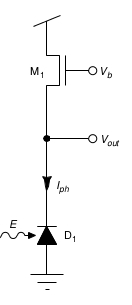
\includegraphics[scale=0.8]{pics/photoreceptor_log.jpg}
  \caption{Photosensors with logarithmic irradiance-to-voltage conversion consisting of a photodiode and a MOSFET in source-follower configuration \cite{book:VLSI}.}
  \label{fig:photoreceptor_log}
\end{figure} 

The differences between supposedly identical receptor outputs are as large as the typical signals
variations produced by real scenes -- circuit is unusable. Hence the necessity for adaptation in a feedback loop, to deal with the circuit mismatch problem (see fig. \ref{fig:photoreceptor_adaptive}).


\begin{figure}[htbp]
  \centering
  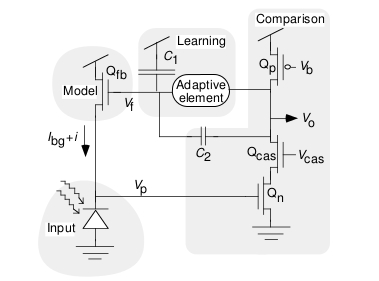
\includegraphics[scale=0.8]{pics/photoreceptor_adaptive.jpg}
  \caption{Adaptive receptor circuit \cite{paper:photo}.}
  \label{fig:photoreceptor_adaptive}
\end{figure} 

\textit{Briefly: The feedback amplifier and the input fight to control the source voltage of $Q_{fb}$, but the feedback amplifier wins because it has much higher gain. The input voltage $v_p$ moves enough so that the output voltage $v_o$ moves enough so that $v_f$ moves enough so that $v_p$ is held nearly clamped. }

The photocurrents are proportional to the areas of the corresponding photodiode junctions, whose spatial variations are the main source
of photocurrent mismatches of identically designed photosensing elements resulting in \textit{fixed-pattern noise}.

The FPN can be reduced by individual tuning of each photosensor. A more economic solution is the enhancement
of transient signals with respect to the mismatched steady-state signals using a
well-matched amplifier stage (capacitive-devider). Adaptation to the DC value can be provided by a resistive element \cite{book:VLSI}.

Adaptive element (see fig. \ref{fig:photo_adaptive_element_schematic}) has current-voltage relationship as shown in the fig. \ref{fig:photo_adaptive_element}.

\begin{figure}[htbp]
\centering
  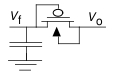
\includegraphics[scale=0.8]{pics/photo_adaptive_element_schematic.jpg}
  \caption{Expansive adaptive element with the capacitor that stores the adaptation state \cite{paper:photo}.}
  \label{fig:photo_adaptive_element_schematic}
\end{figure} 

\begin{figure}[htbp]
  \centering
  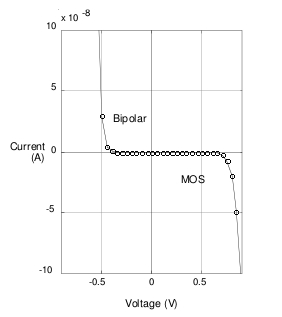
\includegraphics[scale=0.8]{pics/photo_adaptive_element.jpg}
  \caption{Measured current–voltage relationship for the adaptive element. The voltage scale changes logarithmically with the current scale \cite{paper:photo}.}
  \label{fig:photo_adaptive_element}
\end{figure} 


Due to the use of an adaptive element with an expansive nonlinearity there is different respond to input:

\begin{itemize}
\item Large changes (high frequencies, huge changes in illumination, ambient lighting, background change -- from shadow into sunlight) adapt rapidly.  Low gain for static signals (including circuit mismatches) --  the feedback is a short circuit across the adaptive element.
%, and $v_o$ does not need to move much to hold $v_p$ clamped. ??????????????????????????????????????????????????only once instead back of back and forth
\item Small signals around an adaptation point (small contrast variation) adapt slowly. The transient gain of the receptor is high, set by the capacitive-divider ratio as no charge flows through the adaptive element, changes in $v_o$ are coupled to $v_f$ through the capacitive divider \cite{paper:photo}.
\end{itemize}

The amplitude of the response to the
small contrast variation is almost invariant
to the absolute intensity (as in retina in eye), owing to the logarithmic response property. 



\subsection{How you can build a fast logarithmic current-sense amplifier, by using feedback to make a virtual ground?}

To make a virtual ground -- to clamp voltage $V_s$ to constant level.

 $V_s$ node is output of the source-follower log receptor with high parasitic capacitance -- requiring a lot of time to charge or discharge it -- circuit is not responding to high frequencies.  By decoupling output node from the $V_s$ node we get higher bandwidth (grater passband of frequencies).
Hence the necessity for active feedback, to deal with the problem of slow response  \cite{paper:photo}. For the circuit schematic see fig. \ref{fig:photosensor_feedback}

\begin{figure}[htbp]
  \centering
  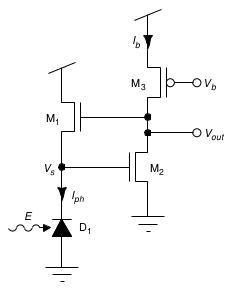
\includegraphics[scale=0.8]{pics/photosensor_feedback.jpg}
  \caption{Logarithmic photosensor with feedback loop icreasing the bandwidth by clamping the voltage $V_s$ \cite{paper:photo}.}
  \label{fig:photosensor_feedback}
\end{figure} 

The voltage output signal then appears at the gate of the MOSFET $M_1$, while the source and therefore the
voltage across the photodiode is practically clamped. The source node drives $V_s$ a two-transistor inverting amplifier
with a pFET current source clamping $V_s$ \cite{book:VLSI}. 

\subsection{How you can use a capacitive divider in the feedback loop of an amplifier to set gain?}

The mismatches can be reduced by a well-matched transient gain stage fabricated with a capacitive divider.

On short time scales , no charge flows through the adaptive element, but changes in $v_o$ are coupled to $v_f$ through the capacitive divider (see fig. \ref{fig:photoreceptor_adaptive}). The transient gain of the receptor is thus set by the capacitive-divider ratio. 
\begin{equation}
A_c = \frac{C_1+C_2}{C_2}, ~~~ \delta V_{out}=A_c A \delta V_s
\end{equation}
The larger $C_1$ is relative to $C_2$, the larger the gain of the circuit \cite{book:VLSI}.

\subsection{How you can use a cascode configuration to increase effective drain resistance?}

If we take a cascode with 2 nFET transistors and name the upper one $M_c$ and the lower one $M_2$ and take variables $g_{dc}, g_{sc}$ -- drain and source, output, input transconductance of $M_c$, $g_{d2}$ -- drain, output transcondunctance of $M_2$ and $g_0$ -- overall conductance of the cascode, $V_x$ -- common node between 2 transistors we can write:
\begin{equation}
g_0 = \frac{\delta}{V_0},
\end{equation}
\begin{equation}
\delta = g_0 V_0 = g_{d2} V_0 - g_{sc} V_x,
\end{equation}
\begin{equation}
( g_{d2} + g_{sc} )V_x = g_{dc} V_0.
\end{equation}

Excluding unknown $V_x$ from both equation we get:
\begin{equation}
\delta = \frac{g_{d2} g_{dc} }{g_{d2} + g_{sc} } V_0 \approx  \frac{g_{d2} g_{dc} }{g_{d2} + g_{sc} } V_0.
\end{equation}
\begin{equation}
g_{0} = g_{d2} \frac{g_{dc}}{g_{sc}} \approx g_{d2} \frac{U_{T}}{V_{e}}.
\end{equation}

And finally we can derive the expression for the change resistance after connecting additional transistor in cascode configuration:
\begin{equation}
r_{0} = r_{d2} \frac{V_{e}}{U_{T}}.
\end{equation}
As we can see, the resistance will be increased by approximately $\frac{V_e}{U_T} \gg 1$.

\subsection{What is the Miller effect?}

The Miller effect occurs when a capacitor feeds back the output of an inverting, high gain amplifier back to the input. If the input needs to move a certain amount, it must charge not only its own side of the capacitor, but also the other side of the capacitor which moves $A$ times as much in the opposite direction. Hence a small capacitance $C$ looks like a capacitance $(A+1)C$ to the input. Since $A \gg 1$, we usually ignore the $1$. The Miller capacitors $C_n$  (see fig. \ref{fig:photoreceptor_adaptive}) from the gate to the drain of $Q_n$ has a substantial effect on the time-response of the receptor. The Miller effect increases the relevant gate–drain and gate–source capacitances by a factor of A  \cite{paper:photo}.

\subsection{How can a cascode be used to reduce it?}

The parasitic capacitance $C_p$ from the source of $M_1$ onto the output node via the gate-to-drain capacitance of nFET $M_2$ gives rise to the Miller effect (see fig. \ref{fig:photosensor_cascode}).

\begin{figure}[htbp]
  \centering
  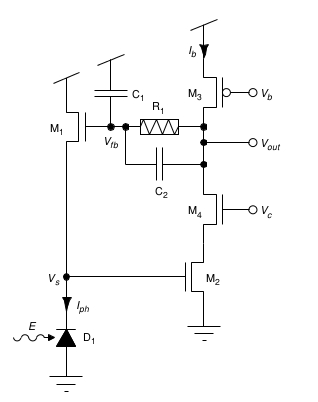
\includegraphics[scale=0.8]{pics/photosensor_cascode.jpg}
  \caption{Adaptive logarithmic photosensor with cascode transistor increasing the bandwidth for small photocurrents \cite{book:VLSI}.}
  \label{fig:photosensor_cascode}
\end{figure} 

Hereby, the apparent capacitance, as seen from the source of $M_1$ , is increased by $C_p$ multiplied by the voltage gain from gate to source. For small photocurrents this effect leads to limited response band width ($I = C \frac{\delta V}{dt}$). The introduction of a cascode with a fixed gate voltage $V_c$ clamps the voltage on the drain of $M_2$, because the current through the amplifier is approximately constant, and largely nullifies the Miller effect (parasitic capacitance has only influence on feedback for changing voltage). 

However, for certain biasing conditions the presence of the cascode can make the circuit unstable \cite{book:VLSI}.
\end{document}